\documentclass[12pt]{article}

\usepackage[margin=1in]{geometry}
\usepackage{amsmath,amssymb}
\usepackage{tikz}
\usetikzlibrary{positioning, arrows.meta, shapes.geometric, fit, calc, backgrounds}
\usepackage{hyperref}
\usepackage{natbib}
\usepackage{booktabs}
\usepackage{caption}
\usepackage{subcaption}
\usepackage{float}
\usepackage{graphicx}

\bibliographystyle{plainnat}

\title{
\textbf{CSCE 775: Deep Reinforcement Learning and Search} \\[0.5em]
\Large RL-Driven Scene Program Synthesis for \\
Synthetic Marine Radar Augmentation
}

\author{
J.C. Vaught
}

\date{February 13, 2026}

\begin{document}

\maketitle

% ============================================================
% INTRODUCTION
% ============================================================
\section{Introduction}

Training robust object detectors for marine radar requires large, diverse labeled datasets, yet collecting and annotating real-world radar scans is expensive, dangerous, and constrained by geography and weather. The EchoTrails framework addresses this by generating synthetic training data from real radar ingredients. Rather than simulating radar physics, EchoTrails composites real extracted echo signatures---target patches previously detected via DBSCAN from vessel-containing radar frames---onto real FURUNO marine radar backgrounds from Charleston harbor. These composited frames are then augmented with a temporal rendering step called \textit{echo trail rendering}, which composites $N$ historical frames with decay-weighted intensity to encode motion information into the training images. A YOLOv8n detector trained on these augmented images learns to distinguish stationary from moving maritime targets based on their trail signatures.

Critically, the EchoTrails generator is not a simple parameter dial. It accepts a full \textit{scene program}: a YAML configuration that specifies the exact number and composition of object groups, each with independently configurable motion paths (fixed positions, linear headings, quadratic B\'{e}zier curves, multi-waypoint splines with cubic interpolation, or arbitrary parametric equations), per-frame intensity profiles (constant, ramping, sinusoidal, or custom mathematical expressions), scripted flicker schedules (a state machine with configurable on/off durations, transition probabilities, and intensity drops), placement constraints (margin from land boundaries, edge preference, per-object land/water mask overrides), and object size filtering. On top of this, the trail renderer itself exposes four categorical axes: decay function (linear, exponential, concave, step), intensity encoding (binary, proportional), color mapping (monochrome, two-tone, gradient, intensity-mapped), and trail length $N$. Clutter generation adds further dimensions: streak count, intensity range, and per-frame randomization. Because the generator supports variable numbers of object groups, variable-length waypoint lists, and arbitrary mathematical expressions for motion and intensity, the configuration space is combinatorially explosive and effectively infinite. Multiple shorter scenes can also be composed within a single generation run, further expanding the space. The existing ablation study evaluates trail length $N$ in isolation while holding all other parameters fixed, leaving the vast joint optimization landscape unexplored. We propose using deep reinforcement learning to learn a policy that \textit{generates scene programs}---composing object groups, trajectories, intensity profiles, flicker schedules, and trail rendering settings---to maximize downstream detection performance.

% ============================================================
% BACKGROUND
% ============================================================
\section{Background: EchoTrails Generator and Detection Pipeline}

The EchoTrails generation pipeline operates in four stages, illustrated in Figure~\ref{fig:pipeline}. First, the system loads three ingredients: 280 real FURUNO radar background frames stored as polar-coordinate CSVs (720 azimuth pulses $\times$ 868 range bins), a library of 5,106 real extracted echo signatures (small 2D intensity patches with metadata including area, intensity statistics, and category), and polygon annotations defining water and land regions. A binary water mask is constructed from these annotations and converted to polar coordinates via a precomputed lookup table (LUT).

\begin{figure}[H]
\centering

\includegraphics[width=\textwidth]{figures/fig_pipeline.pdf}
\caption{The EchoTrails pipeline. The RCS (Radar Cross-Section) simulator generates raw PPI (Plan Position Indicator) frames by compositing real echo signatures onto real radar backgrounds. The trail renderer applies temporal augmentation with configurable parameters $N$ (trail length), $f(k)$ (decay function), encoding mode, and color mapping. A YOLOv8 detector is trained on the trailed images and evaluated by mAP$_{50}$.}
\label{fig:pipeline}
\end{figure}

Second, a scene program (YAML configuration) specifies the composition of each scene. For each object group, the generator filters the library by size and category, generates motion paths via one of five path types, creates an intensity engine combining a base profile with random jitter and an optional flicker state machine, and assembles a per-frame placement plan. Each frame plan specifies which background to use (backgrounds cycle through the 280 available frames), and a list of object placements with polar coordinates, dimensions, class IDs, and echo data. Objects are composited onto the background in polar space using max-blending---echo values never overwrite existing signal, they only add on top. Synthetic clutter can be injected as radial streaks with range-dependent width (wide near the radar, narrow at distance) and raised cosine intensity envelopes. Figure~\ref{fig:scene_preview} shows a representative scene with stationary, slow, medium, and fast object trajectories overlaid on the Charleston harbor water mask.

\begin{figure}[H]
\centering
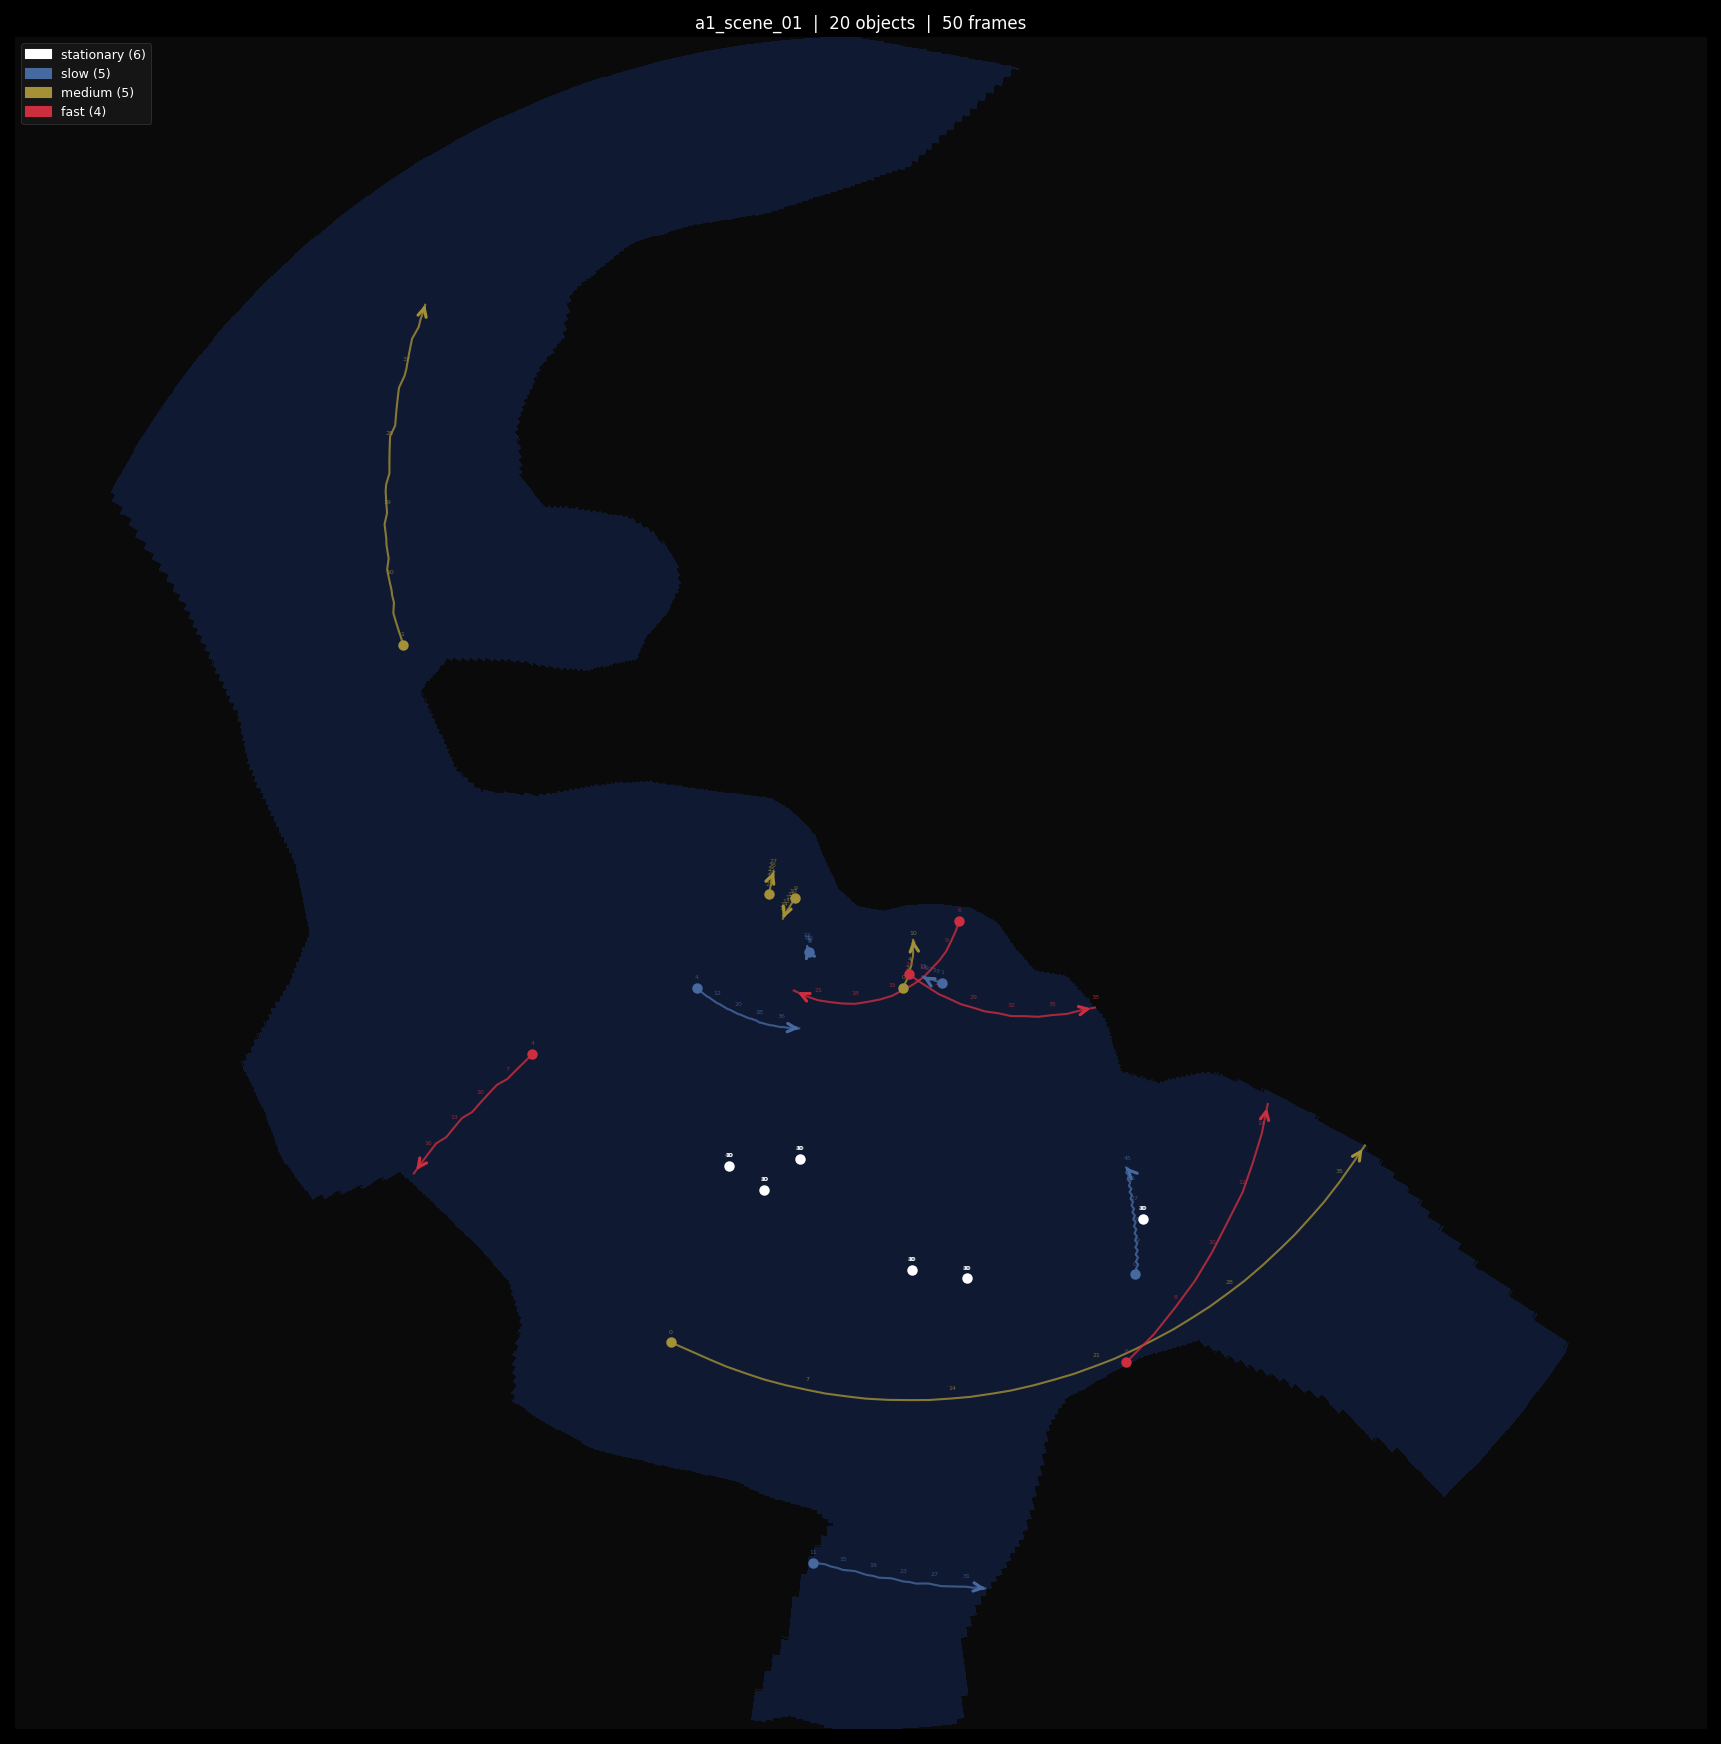
\includegraphics[width=0.7\textwidth]{figures/fig_scene_preview.png}
\caption{Scene preview for a representative EchoTrails configuration showing 20 objects across 50 frames. White dots indicate stationary targets. Colored paths show moving targets at slow (blue), medium (yellow), and fast (red) speeds. The dark blue region is the water mask derived from Charleston harbor annotations. Each trajectory is independently configurable with its own path type, speed, duration, intensity profile, and flicker schedule.}
\label{fig:scene_preview}
\end{figure}

Third, the composited polar frames are converted to 1735$\times$1735 Cartesian grayscale images using the precomputed LUT. YOLO-format bounding box labels are generated automatically: each polar bounding box's four corners are projected to Cartesian coordinates, and an axis-aligned bounding box is computed and normalized by image size. Finally, the echo trail renderer composites $N$ historical frames onto each output image using per-pixel MAX blending with a configurable decay function $f(k)$ that weights history frame $k$ by age, an intensity encoding that determines whether pixel weight is binary (any nonzero pixel gets full weight) or proportional (weight scales with original intensity), and a color mapping that encodes temporal information visually. Figure~\ref{fig:splash} illustrates how different decay functions affect the trail appearance for a single moving target, and Figure~\ref{fig:clutter} shows the impact of trail rendering under increasing clutter conditions. The detection task is binary classification---stationary (class 0) versus moving (class 1)---evaluated by training a YOLOv8n detector for 50 epochs at image size 640 with batch size 16.

\begin{figure}[H]
\centering
\begin{subfigure}[t]{0.48\textwidth}
\centering
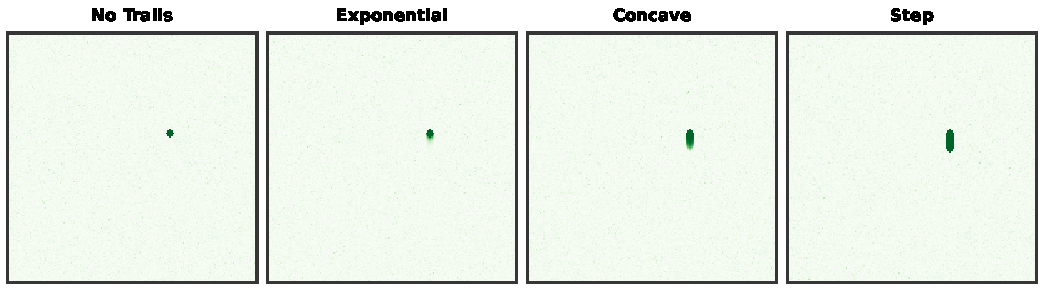
\includegraphics[width=\textwidth]{figures/fig_trail_examples.pdf}
\caption{Effect of decay function on trail appearance. From left: no trails, exponential decay (fast initial drop), concave decay (holds intensity then sharp drop), and step decay (uniform weight, hard cutoff).}
\label{fig:splash}
\end{subfigure}
\hfill
\begin{subfigure}[t]{0.48\textwidth}
\centering
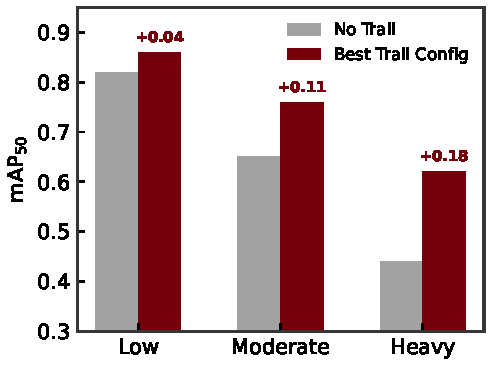
\includegraphics[width=\textwidth]{figures/fig_clutter.pdf}
\caption{Detection improvement from trail rendering under increasing clutter. The mAP$_{50}$ gap between no-trail and best-trail configurations widens from $+0.04$ at low clutter to $+0.18$ at heavy clutter, demonstrating that trails become more valuable as conditions degrade.}
\label{fig:clutter}
\end{subfigure}
\caption{Trail rendering effects and clutter interaction from the EchoTrails ablation study.}
\label{fig:trail_and_clutter}
\end{figure}

% ============================================================
% APPROACH
% ============================================================
\section{Approach}

We formulate scene program synthesis as a Markov Decision Process (MDP). At each step $t$, the agent observes a state $\boldsymbol{s}_t = (\boldsymbol{\theta}_t, \boldsymbol{m}_t)$ comprising the current scene program configuration $\boldsymbol{\theta}_t$ and recent validation metrics $\boldsymbol{m}_t$ (mAP$_{50\text{-}95}$, precision, recall from the previous $h$ evaluation rounds). The agent then outputs an action $\boldsymbol{a}_t$ specifying a new scene program. This action is structured and hierarchical: top-level decisions include the number of object groups, trail rendering parameters ($N$, decay type, intensity encoding, color mapping), and clutter settings (streak count, intensity bounds). For each object group, the agent specifies a path type, and conditional on that choice, the path-specific parameters: coordinates or headings for linear paths, control points and curvature for B\'{e}zier paths, waypoint sequences for spline paths, or mathematical expressions for parametric paths. The agent also sets per-group intensity profiles (base multiplier, variability, profile type, and if sinusoidal, the period and amplitude), flicker schedules (rate, on/off durations, intensity drop), placement constraints (margin, edge preference), object count, and size range. Because the generator supports variable-length waypoint lists and arbitrary expressions, the action space is not a fixed-dimensional vector but a variable-length structured program. Categorical choices (path type, decay function, color mapping, intensity encoding, profile type) are parameterized as logits and sampled via Gumbel-Softmax to enable gradient flow. The reward $r_t$ is the validation mAP$_{50\text{-}95}$ achieved by a YOLOv8n detector trained on data generated from the proposed scene program. We adopt Soft Actor-Critic (SAC) \citep{Haarnoja2018SAC} for its off-policy sample efficiency---critical when each environment step requires a full generate-train-evaluate cycle of approximately 2,500 frames and 50 training epochs---and its maximum entropy objective, which naturally encourages diverse scene program exploration and guards against premature convergence to a single configuration.

Our approach differs from prior work in several respects. Unlike static domain randomization \citep{Tobin2017DomainRandomization, Tremblay2018TrainingDNN}, which samples augmentation parameters from a fixed distribution, our policy adapts scene programs online in response to downstream detection performance. Unlike AutoAugment \citep{Cubuk2019AutoAugment}, which searches over a flat space of image-level transforms, our agent composes structured, multi-object scene programs with conditional parameters and variable length. Unlike Meta-Sim \citep{Kar2019MetaSim}, which learns a distribution over a fixed scene graph, our configuration space includes arbitrary mathematical expressions and variable-length waypoint sequences, making it closer to program synthesis than parameter optimization. Unlike Active Domain Randomization \citep{Mehta2020ActiveDR}, which searches for maximally informative randomization ranges, our formulation directly optimizes the downstream detection objective. Finally, our generator uniquely operates on real echo data and real radar backgrounds rather than physics simulation, so the RL agent is optimizing how to \textit{present and modulate real signal} rather than how to \textit{approximate physical fidelity}.

% ============================================================
% FIGURE: SYSTEM ARCHITECTURE
% ============================================================
\begin{figure}[H]
\centering
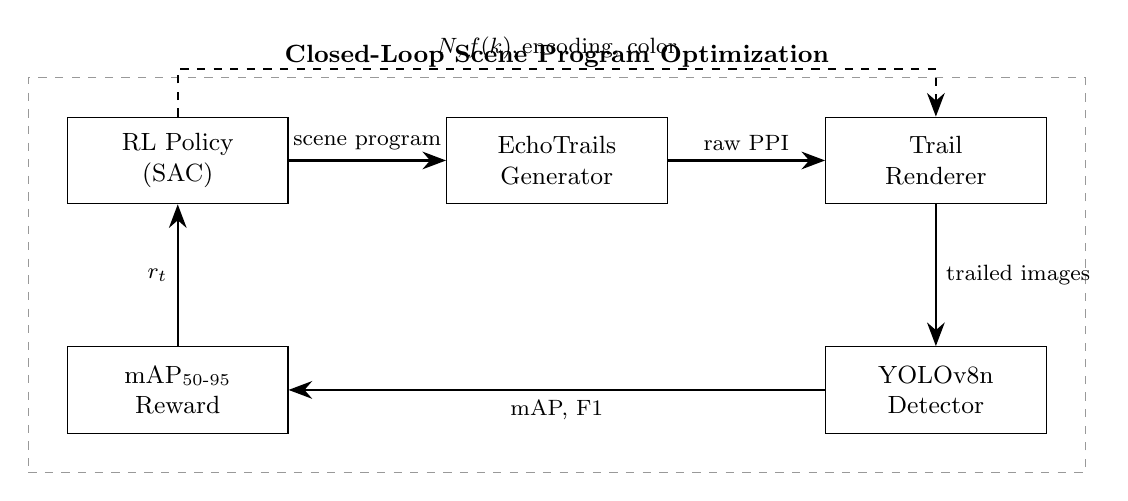
\begin{tikzpicture}[
    block/.style={draw, minimum width=2.8cm, minimum height=1.1cm, align=center, font=\small},
    data/.style={draw, minimum width=2.2cm, minimum height=0.9cm, align=center, font=\small, dashed},
    arr/.style={-{Stealth[length=3mm]}, thick},
    every node/.style={font=\small}
]

% RL Agent
\node[block, fill=white] (agent) {RL Policy\\(SAC)};

% Generator
\node[block, fill=white, right=2.0cm of agent] (gen) {EchoTrails\\Generator};

% Trail Renderer
\node[block, fill=white, right=2.0cm of gen] (trail) {Trail\\Renderer};

% Downstream Model
\node[block, fill=white, below=1.8cm of trail] (model) {YOLOv8n\\Detector};

% Validation Score
\node[block, fill=white, below=1.8cm of agent] (val) {mAP$_{50\text{-}95}$\\Reward};

% Arrows
\draw[arr] (agent) -- node[above, font=\footnotesize] {scene program} (gen);
\draw[arr] (gen) -- node[above, font=\footnotesize] {raw PPI} (trail);
\draw[arr] (trail) -- node[right, font=\footnotesize] {trailed images} (model);
\draw[arr] (model) -- node[below, font=\footnotesize] {mAP, F1} (val);
\draw[arr] (val) -- node[left, font=\footnotesize] {$r_t$} (agent);

% Curved arrow for trail params
\draw[arr, dashed] (agent.north) -- ++(0,0.6) -| node[above, pos=0.25, font=\footnotesize] {$N, f(k), \text{encoding, color}$} (trail.north);

% Background box
\begin{scope}[on background layer]
\node[draw=black!40, dashed, inner sep=14pt, fit=(agent)(gen)(trail)(model)(val), label={[font=\small\bfseries]above:Closed-Loop Scene Program Optimization}] {};
\end{scope}

\end{tikzpicture}
\caption{Proposed system architecture. The SAC policy outputs both a structured scene program (object groups, paths, intensity profiles, flicker schedules, clutter settings) and trail rendering parameters ($N$, decay $f(k)$, encoding, color mapping). The EchoTrails generator produces raw PPI frames, which the trail renderer augments with temporal compositing. A YOLOv8n detector is trained on the augmented images and its validation mAP$_{50\text{-}95}$ serves as the reward signal, closing the loop.}
\label{fig:system_arch}
\end{figure}

% ============================================================
% EVALUATION
% ============================================================
\section{Evaluation}

We evaluate using the EchoTrails dataset infrastructure. The existing dataset comprises 10 scenes of 50 frames each, split 9:1 for training and validation, with approximately 50 objects per scene stratified across seven groups: stationary targets, slow movers (2~px/frame), medium movers (5~px/frame), and fast movers (12~px/frame), each originating from edge or interior positions. All scenes use real Charleston harbor radar backgrounds with the 5,106-object echo library. Two clutter conditions are tested: scenes with synthetic clutter (100 streaks per frame, intensity 200--255) and scenes without clutter. The primary metric is mAP$_{50\text{-}95}$ (mean average precision averaged over IoU thresholds 0.50 to 0.95), with secondary metrics including mAP$_{50}$, precision, recall, and F1 score. We additionally report per-speed-tier detection rates (slow, medium, fast) to assess whether the RL-discovered scene programs improve detection uniformly or favor particular motion regimes.

We compare against four baselines. The first uses the best configuration identified by the existing single-variable ablation study: $N = 20$ with linear decay, proportional intensity encoding, and two-tone color mapping, with all scene composition parameters at their default values. The second replaces the RL policy with uniform random sampling over the full scene program space, generating 100 random configurations and reporting the best. The third substitutes Bayesian optimization (Gaussian process with expected improvement acquisition) operating over a flattened subset of the parameter space, given the same computational budget as the RL agent. The fourth uses no echo trails at all ($N = 0$, grayscale-to-RGB conversion), establishing the lower bound of detection performance without temporal augmentation. We additionally conduct ablation studies that restrict the RL agent's action space to subsets of the full scene program---for example, fixing the scene composition and optimizing only trail rendering parameters, or vice versa---to quantify the contribution of joint optimization versus the individual parameter groups.

% ============================================================
% CONCLUSION
% ============================================================
\section{Conclusion}

We propose a reinforcement learning framework for synthesizing scene programs that jointly optimize the full parameter space of the EchoTrails synthetic marine radar augmentation pipeline. The generator's expressiveness---supporting exact coordinate placement, multi-waypoint trajectories, parametric motion equations, scripted flicker schedules, per-object land/water mask overrides, and composable multi-scene runs---makes the configuration space effectively infinite, far beyond the reach of manual tuning or grid search. By formulating scene program synthesis as an MDP and solving it with SAC, our approach replaces single-variable ablation with a closed-loop adaptive search that can discover interaction effects between trail rendering, clutter, motion, and intensity parameters that isolated sweeps cannot capture. The evaluation plan compares against the ablation-best configuration, random search, Bayesian optimization, and no-trail baselines across clutter conditions, unseen scene layouts, and per-speed-tier detection scenarios.

% ============================================================
% REFERENCES
% ============================================================
\bibliography{references}
\nocite{*}

\end{document}
